% Created by tikzDevice version 0.12.6 on 2024-09-26 13:54:40
% !TEX encoding = UTF-8 Unicode
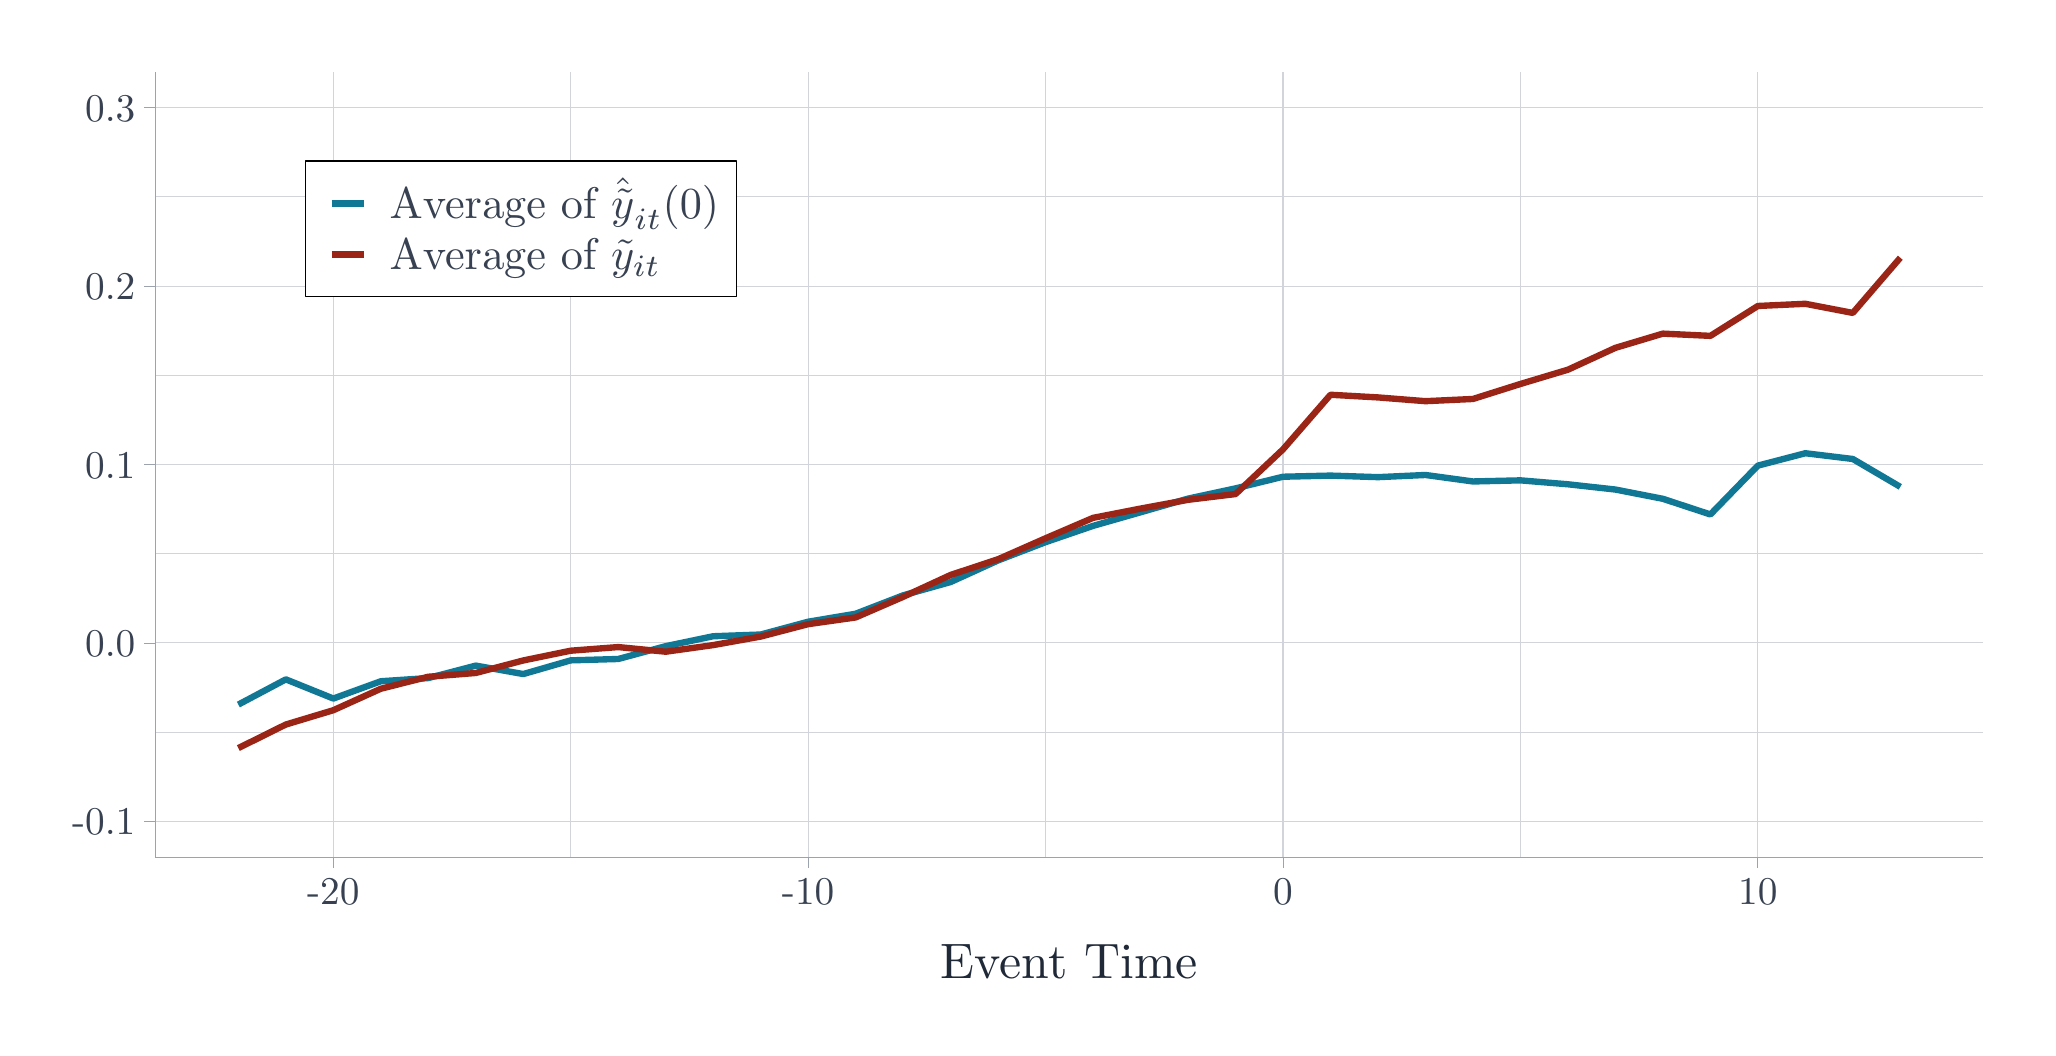
\begin{tikzpicture}[x=1pt,y=1pt]
\definecolor{fillColor}{RGB}{255,255,255}
\path[use as bounding box,fill=fillColor] (0,0) rectangle (722.70,361.35);
\begin{scope}
\path[clip] (  0.00,  0.00) rectangle (722.70,361.35);
\definecolor{drawColor}{RGB}{255,255,255}

\path[draw=drawColor,line width= 0.8pt,line join=round,line cap=round,fill=fillColor] (  0.00,  0.00) rectangle (722.70,361.35);
\end{scope}
\begin{scope}
\path[clip] ( 46.10, 61.65) rectangle (706.70,345.35);
\definecolor{drawColor}{RGB}{255,255,255}
\definecolor{fillColor}{RGB}{255,255,255}

\path[draw=drawColor,line width= 0.8pt,line join=round,line cap=round,fill=fillColor] ( 46.10, 61.65) rectangle (706.70,345.35);
\definecolor{drawColor}{RGB}{209,213,219}

\path[draw=drawColor,line width= 0.4pt,line join=round] ( 46.10,106.79) --
	(706.70,106.79);

\path[draw=drawColor,line width= 0.4pt,line join=round] ( 46.10,171.26) --
	(706.70,171.26);

\path[draw=drawColor,line width= 0.4pt,line join=round] ( 46.10,235.74) --
	(706.70,235.74);

\path[draw=drawColor,line width= 0.4pt,line join=round] ( 46.10,300.22) --
	(706.70,300.22);

\path[draw=drawColor,line width= 0.4pt,line join=round] (196.24, 61.65) --
	(196.24,345.35);

\path[draw=drawColor,line width= 0.4pt,line join=round] (367.82, 61.65) --
	(367.82,345.35);

\path[draw=drawColor,line width= 0.4pt,line join=round] (539.41, 61.65) --
	(539.41,345.35);

\path[draw=drawColor,line width= 0.4pt,line join=round] ( 46.10, 74.55) --
	(706.70, 74.55);

\path[draw=drawColor,line width= 0.4pt,line join=round] ( 46.10,139.03) --
	(706.70,139.03);

\path[draw=drawColor,line width= 0.4pt,line join=round] ( 46.10,203.50) --
	(706.70,203.50);

\path[draw=drawColor,line width= 0.4pt,line join=round] ( 46.10,267.98) --
	(706.70,267.98);

\path[draw=drawColor,line width= 0.4pt,line join=round] ( 46.10,332.45) --
	(706.70,332.45);

\path[draw=drawColor,line width= 0.4pt,line join=round] (110.45, 61.65) --
	(110.45,345.35);

\path[draw=drawColor,line width= 0.4pt,line join=round] (282.03, 61.65) --
	(282.03,345.35);

\path[draw=drawColor,line width= 0.4pt,line join=round] (453.61, 61.65) --
	(453.61,345.35);

\path[draw=drawColor,line width= 0.4pt,line join=round] (625.20, 61.65) --
	(625.20,345.35);
\definecolor{drawColor}{RGB}{16,120,149}

\path[draw=drawColor,line width= 2.3pt,line join=round] ( 76.13,116.75) --
	( 93.29,125.86) --
	(110.45,118.93) --
	(127.61,125.18) --
	(144.76,126.33) --
	(161.92,130.83) --
	(179.08,127.78) --
	(196.24,132.73) --
	(213.40,133.22) --
	(230.56,137.86) --
	(247.71,141.44) --
	(264.87,142.06) --
	(282.03,146.69) --
	(299.19,149.57) --
	(316.35,156.22) --
	(333.51,161.03) --
	(350.66,168.84) --
	(367.82,175.44) --
	(384.98,181.32) --
	(402.14,186.23) --
	(419.30,191.17) --
	(436.46,194.87) --
	(453.61,199.08) --
	(470.77,199.49) --
	(487.93,198.93) --
	(505.09,199.71) --
	(522.25,197.37) --
	(539.41,197.77) --
	(556.56,196.35) --
	(573.72,194.45) --
	(590.88,191.10) --
	(608.04,185.45) --
	(625.20,203.09) --
	(642.36,207.57) --
	(659.51,205.49) --
	(676.67,195.42);
\definecolor{drawColor}{RGB}{154,36,21}

\path[draw=drawColor,line width= 2.3pt,line join=round] ( 76.13,101.03) --
	( 93.29,109.54) --
	(110.45,114.71) --
	(127.61,122.47) --
	(144.76,126.80) --
	(161.92,128.17) --
	(179.08,132.69) --
	(196.24,136.22) --
	(213.40,137.53) --
	(230.56,135.85) --
	(247.71,138.24) --
	(264.87,141.32) --
	(282.03,145.81) --
	(299.19,148.23) --
	(316.35,155.67) --
	(333.51,163.59) --
	(350.66,169.27) --
	(367.82,176.84) --
	(384.98,184.22) --
	(402.14,187.57) --
	(419.30,190.74) --
	(436.46,192.82) --
	(453.61,208.97) --
	(470.77,228.70) --
	(487.93,227.74) --
	(505.09,226.38) --
	(522.25,227.18) --
	(539.41,232.60) --
	(556.56,237.75) --
	(573.72,245.65) --
	(590.88,250.79) --
	(608.04,249.98) --
	(625.20,260.78) --
	(642.36,261.57) --
	(659.51,258.27) --
	(676.67,278.21);
\end{scope}
\begin{scope}
\path[clip] (  0.00,  0.00) rectangle (722.70,361.35);
\definecolor{drawColor}{RGB}{156,163,175}

\path[draw=drawColor,line width= 0.3pt,line join=round] ( 46.10, 61.65) --
	( 46.10,345.35);
\end{scope}
\begin{scope}
\path[clip] (  0.00,  0.00) rectangle (722.70,361.35);
\definecolor{drawColor}{RGB}{55,65,81}

\node[text=drawColor,anchor=base east,inner sep=0pt, outer sep=0pt, scale=  1.42] at ( 38.90, 69.65) {-0.1};

\node[text=drawColor,anchor=base east,inner sep=0pt, outer sep=0pt, scale=  1.42] at ( 38.90,134.13) {0.0};

\node[text=drawColor,anchor=base east,inner sep=0pt, outer sep=0pt, scale=  1.42] at ( 38.90,198.61) {0.1};

\node[text=drawColor,anchor=base east,inner sep=0pt, outer sep=0pt, scale=  1.42] at ( 38.90,263.08) {0.2};

\node[text=drawColor,anchor=base east,inner sep=0pt, outer sep=0pt, scale=  1.42] at ( 38.90,327.56) {0.3};
\end{scope}
\begin{scope}
\path[clip] (  0.00,  0.00) rectangle (722.70,361.35);
\definecolor{drawColor}{RGB}{156,163,175}

\path[draw=drawColor,line width= 0.3pt,line join=round] ( 42.10, 74.55) --
	( 46.10, 74.55);

\path[draw=drawColor,line width= 0.3pt,line join=round] ( 42.10,139.03) --
	( 46.10,139.03);

\path[draw=drawColor,line width= 0.3pt,line join=round] ( 42.10,203.50) --
	( 46.10,203.50);

\path[draw=drawColor,line width= 0.3pt,line join=round] ( 42.10,267.98) --
	( 46.10,267.98);

\path[draw=drawColor,line width= 0.3pt,line join=round] ( 42.10,332.45) --
	( 46.10,332.45);
\end{scope}
\begin{scope}
\path[clip] (  0.00,  0.00) rectangle (722.70,361.35);
\definecolor{drawColor}{RGB}{156,163,175}

\path[draw=drawColor,line width= 0.3pt,line join=round] ( 46.10, 61.65) --
	(706.70, 61.65);
\end{scope}
\begin{scope}
\path[clip] (  0.00,  0.00) rectangle (722.70,361.35);
\definecolor{drawColor}{RGB}{156,163,175}

\path[draw=drawColor,line width= 0.3pt,line join=round] (110.45, 57.65) --
	(110.45, 61.65);

\path[draw=drawColor,line width= 0.3pt,line join=round] (282.03, 57.65) --
	(282.03, 61.65);

\path[draw=drawColor,line width= 0.3pt,line join=round] (453.61, 57.65) --
	(453.61, 61.65);

\path[draw=drawColor,line width= 0.3pt,line join=round] (625.20, 57.65) --
	(625.20, 61.65);
\end{scope}
\begin{scope}
\path[clip] (  0.00,  0.00) rectangle (722.70,361.35);
\definecolor{drawColor}{RGB}{55,65,81}

\node[text=drawColor,anchor=base,inner sep=0pt, outer sep=0pt, scale=  1.42] at (110.45, 44.66) {-20};

\node[text=drawColor,anchor=base,inner sep=0pt, outer sep=0pt, scale=  1.42] at (282.03, 44.66) {-10};

\node[text=drawColor,anchor=base,inner sep=0pt, outer sep=0pt, scale=  1.42] at (453.61, 44.66) {0};

\node[text=drawColor,anchor=base,inner sep=0pt, outer sep=0pt, scale=  1.42] at (625.20, 44.66) {10};
\end{scope}
\begin{scope}
\path[clip] (  0.00,  0.00) rectangle (722.70,361.35);
\definecolor{drawColor}{RGB}{31,41,55}

\node[text=drawColor,anchor=base,inner sep=0pt, outer sep=0pt, scale=  1.80] at (376.40, 17.75) {Event Time};
\end{scope}
\begin{scope}
\path[clip] (  0.00,  0.00) rectangle (722.70,361.35);
\definecolor{drawColor}{RGB}{0,0,0}
\definecolor{fillColor}{RGB}{255,255,255}

\path[draw=drawColor,line width= 0.6pt,line join=round,line cap=round,fill=fillColor] (100.36,264.16) rectangle (256.09,313.06);
\end{scope}
\begin{scope}
\path[clip] (  0.00,  0.00) rectangle (722.70,361.35);
\definecolor{drawColor}{RGB}{255,255,255}
\definecolor{fillColor}{RGB}{255,255,255}

\path[draw=drawColor,line width= 0.8pt,line join=round,line cap=round,fill=fillColor] (108.36,290.61) rectangle (122.81,305.06);
\end{scope}
\begin{scope}
\path[clip] (  0.00,  0.00) rectangle (722.70,361.35);
\definecolor{drawColor}{RGB}{16,120,149}

\path[draw=drawColor,line width= 2.3pt,line join=round] (109.81,297.84) -- (121.37,297.84);
\end{scope}
\begin{scope}
\path[clip] (  0.00,  0.00) rectangle (722.70,361.35);
\definecolor{drawColor}{RGB}{255,255,255}
\definecolor{fillColor}{RGB}{255,255,255}

\path[draw=drawColor,line width= 0.8pt,line join=round,line cap=round,fill=fillColor] (108.36,272.16) rectangle (122.81,286.61);
\end{scope}
\begin{scope}
\path[clip] (  0.00,  0.00) rectangle (722.70,361.35);
\definecolor{drawColor}{RGB}{154,36,21}

\path[draw=drawColor,line width= 2.3pt,line join=round] (109.81,279.38) -- (121.37,279.38);
\end{scope}
\begin{scope}
\path[clip] (  0.00,  0.00) rectangle (722.70,361.35);
\definecolor{drawColor}{RGB}{55,65,81}

\node[text=drawColor,anchor=base west,inner sep=0pt, outer sep=0pt, scale=  1.60] at (130.81,292.33) {Average of $\hat{\tilde{y}}_{it}(0)$};
\end{scope}
\begin{scope}
\path[clip] (  0.00,  0.00) rectangle (722.70,361.35);
\definecolor{drawColor}{RGB}{55,65,81}

\node[text=drawColor,anchor=base west,inner sep=0pt, outer sep=0pt, scale=  1.60] at (130.81,273.87) {Average of $\tilde{y}_{it}$};
\end{scope}
\end{tikzpicture}
